% Povinný argument: Kód předmětu
\newcommand{\subject}{BPC-IC1}
% Povinný argument: Název předmětu
\newcommand{\subjectname}{Otázky 2022}
% Povinný argument: Seznam autorů
\newcommand{\authors}{Piesek komputerowy}
% Povinný argument: Seznam korektorů
\newcommand{\corrections}{Nigdo}
% Nepovinný argument: Cílová skupina dokumentu
\newcommand{\docgroup}{Informační bezpečnost, FEKT VUT}

% Přepsáním argumentu na 'false' vypnete balíček 'minted' pro sázení kódu.
% Pro jeho použití lokálně musíte mít v systému dostupný Python 3, python
% knihovnu 'minted' a PDFLaTeX musíte spouštět s argumentem '-shell-escape'.
% Místo něj můžete použít prostředí 'lstlisting'.
\newcommand{\docminted}{true}

% FEKT.tex
% https://github.com/VUT-FEKT-IBE/FEKT.tex
% Git hash repozitáře v době kopírování:

\documentclass[
    % Velikost základního písma je 12 bodů
    12pt,
    % Formát papíru je A4
    a4paper,
    % Oboustranný tisk
    twoside,
    % Záložky a metainformace ve výsledném PDF budou v kódování unicode
    unicode,
]{article}

%%%%%%%%%%%%%%%%%%%%
% OBECNÉ NASTAVENÍ %
%%%%%%%%%%%%%%%%%%%%

% Kódování zdrojových souborů
\usepackage[utf8]{inputenc}
% Kódování výstupního souboru
\usepackage[T1]{fontenc}
% Podpora češtiny
\usepackage[czech]{babel}

% Geometrie stránky
\usepackage[
    % Horní a dolní okraj
    tmargin=25mm,
    bmargin=25mm,
    % Vnitřní a vnější okraj
    lmargin=30mm,
    rmargin=20mm,
    % Velikost zápatí
    footskip=17mm,
    % Vypnutí záhlaví
    nohead,
]{geometry}

% Zajištění kopírovatelnosti a prohledávanosti vytvořených PDF
\usepackage{cmap}
% Podmínky (pro použití v titulní straně)
\usepackage{ifthen}

%%%%%%%%%%%%%%%
% FORMÁTOVÁNÍ %
%%%%%%%%%%%%%%%

% Nastavení stylu nadpisů
\usepackage{sectsty}
% Formátování obsahů
\usepackage{tocloft}
\setcounter{tocdepth}{1}
% Odstranění mezer mezi řádky v seznamech
\usepackage{enumitem}
\setlist{nosep}
\setitemize{leftmargin=1em}
\setenumerate{leftmargin=1.5em}
\renewcommand{\labelitemi}{--}
\renewcommand{\labelitemii}{$\circ$}
\renewcommand{\labelitemiii}{$\cdot$}
\renewcommand{\labelitemiv}{--}
% Sázení správných uvozovek pomocí '\enquote{}'
\usepackage{csquotes}
% Vynucení umístění poznámek pod čarou vespod stránky
\usepackage[bottom]{footmisc}
% Automatické zarovnání textu k předcházení vdov a parchantů
\usepackage[defaultlines=3,all=true]{nowidow}
% Zalomení části textu pokud není na současné stránce dost místa
\usepackage{needspace}
% Nastavení řádkování
\usepackage{setspace}
\onehalfspacing
% Změna odsazení odstavců
\setlength{\parskip}{1em}
\setlength{\parindent}{0em}

% Bezpatkové sázení nadpisů
\allsectionsfont{\sffamily}
% Změna formátování nadpisu a podnadpisů v Obsahu
\renewcommand{\cfttoctitlefont}{\Large\bfseries\sffamily}
\renewcommand{\cftsubsecdotsep}{\cftdotsep}

% Použití moderní/aktualizované sady písem
\usepackage{lmodern}

%%%%%%%%%%%
% NADPISY %
%%%%%%%%%%%

\usepackage{titlesec}

\titlespacing*{\section}{0pt}{10pt}{-0.2\baselineskip}
\titlespacing*{\subsection}{0pt}{0.2\baselineskip}{-0.2\baselineskip}
\titlespacing*{\subsubsection}{0pt}{0.2\baselineskip}{-0.2\baselineskip}
\titlespacing*{\paragraph}{0pt}{0pt}{1em}

%%%%%%%%%%
% ODKAZY %
%%%%%%%%%%

% Tvorba hypertextových odkazů
\usepackage[
    breaklinks=true,
    hypertexnames=false,
]{hyperref}
% Nastavení barvení odkazů
\hypersetup{
    colorlinks,
    citecolor=black,
    filecolor=black,
    linkcolor=black,
    urlcolor=blue
}

%%%%%%%%%%%%%%%%%%%%%%%%%%%
% OBRÁZKY, GRAFY, TABULKY %
%%%%%%%%%%%%%%%%%%%%%%%%%%%

% Vkládání obrázků
\usepackage{graphicx}
\usepackage{subfig}
% Nastavení popisů obrázků, výpisů a tabulek
\usepackage{caption}
\captionsetup{justification=centering}
% Grafy a vektorové obrázky
\usepackage{tikz}
\usetikzlibrary{shapes,arrows}
% Složitější tabulky
\usepackage{tabularx}
\usepackage{multicol}

% Sázení osamocených float prostředí v horní části stránky
\makeatletter
\setlength{\@fptop}{0pt plus 10pt minus 0pt}
\makeatother

% Vynucení vypsání floating prostředí pomocí \FloatBarrier
\usepackage{placeins}

%%%%%%%%%%%%%%
% MATEMATIKA %
%%%%%%%%%%%%%%

% Sázení matematiky a matematických symbolů ('\mathbb{}')
\usepackage{amsmath}
\usepackage{amssymb}
% Sázení fyzikálních veličin
\usepackage{siunitx}

%%%%%%%%%%%%%%%%%
% ZDROJOVÉ KÓDY %
%%%%%%%%%%%%%%%%%

% Sazba zdrojových kódů
\usepackage[formats]{listings}
% Přepnutí prostředí 'code' do režimu výpisu kódu
\newenvironment{code}{\captionsetup{type=listing}}{}

\lstset{
    basicstyle=\small\ttfamily,
    numbers=left,
    numberstyle=\tiny,
    tabsize=4,
    columns=fixed,
    showstringspaces=false,
    showtabs=false,
    keepspaces,
}

% Balíček 'minted' budeme používat pouze pokud je jeho hodnota nastavena na 'true'
\providecommand{\docminted}{false}
\ifthenelse{\equal{\docminted}{true}}
{
    % Sazba zdrojových kódů
    \usepackage[newfloat]{minted}
    % Nastavení barev 'minted' kódů
    \usemintedstyle{pastie}
}
{
    % \docminted není 'true', nic neprovádíme
    % Pokud je v dokumentu 'minted' prostředí, dokument se nepodaří přeložit.
}

%%%%%%%%%%%
% TITULKA %
%%%%%%%%%%%

\IfFileExists{./.repo.tex}{
    % Soubor '.repo.tex' může (re)definovat povinné a nepovinné argumenty
    % souboru 'main.tex'. To lze využít v případech kdy v jednom repozitáři
    % existuje více dokumentů najednou (např. státnicové otázky).
    \input{.repo}
}{}

% Pokud byly nepovinné argumenty zakomentovány nebo vymazány, přidáme prázdné
% definice příkazů, aby bylo dokument možné správně přeložit.
\providecommand{\docdesc}{}
\providecommand{\docgroup}{}
\providecommand{\docurl}{}

\newcommand{\titulka}{
    \vspace*{2em}
    \begin{center}
        {\Huge \bfseries \subject}

        \vspace*{1em}

        {\Huge \bfseries \subjectname}

        \vspace*{2em}

        {\Large \docdesc}

        \vspace*{1em}

        \docgroup

        \url{\docurl}
    \end{center}

    \vfill

    \begin{tabular}{ll}
        Text:      & \authors     \\
        Korektura: & \corrections \\
    \end{tabular}
    \hfill
    \today

    \thispagestyle{empty}
    \newpage
}

\usepackage{mdframed}

\begin{document}

\titulka{}

\tableofcontents
\thispagestyle{empty}

\setcounter{page}{0}

\clearpage
\section{Definice ekonomie a mikroekonomie. Metody ekonomické vědy. Chyby
v ekonomickém způsobu myšlení a uvažování. Racionální chování člověka a úskalí
rozhodovacích procesů.}

\subsection{Ekonomie}
\begin{itemize}
    \item Věda o lidském rozhodování a jednání ve světě omezených zdrojů a neomezených potřeb.
    Věnuje se produkci, rozdělování a spotřebě výrobků a služeb.
\end{itemize}

\subsection{Mikroekonomie}
\begin{itemize}
    \item Analýza chování dílčích ekonomických subjektů: jednotlivců, domácností a firem,
    stav a vývoj jednotlivých trhů (výrobků a služeb, primárních výrobních faktorů).
    \item Otázky jako příklad:
    \begin{itemize}
        \item jak se utváří cena na trhu čaje
        \item jak se mění chování spotřebitele zvýšením ceny benzínu
        \item jaký vliv bude mít na pracovní úsilí lidí vyšší daň ze mzdy
        \item jak se chovají odborové svazy
        \item jak se určuje výroba v jednotlivých firmách, odvětvích apod.
        \item jak jsou určeny mzdy, zisky, úroky a jiné důchody
        \item jak se chová na trhu spotřebitel
        \item jak se projevuje státní politika na změnách výroby, ceny v jednotlivých firmách, na
        konkrétních trzích, atd.
    \end{itemize}
\end{itemize}

\subsection{Metody ekonomické vědy}
\begin{itemize}
    \item analýza (dělení celku na části)
    \item syntéza (skládání myšlenkových částí do celku)
    \item indukce (vytváření obecných pravidel na základě konkrétních příkladů)
    \item dedukce (z předpokladů vyvodíme závěr)
    \item \textbf{téměř není možné} využít metodu experimentu
    \item modely
    \item Metody nejsou univerzální ani zastupitelné, mají různé přednosti a ekonomie je velice komplexní.
\end{itemize}

\subsection{Chyby v ekonomickém způsobu myšlení}
\begin{itemize}
    \item nedodržení pravidla \uv{za jinak stejných podmínek} (ceteris paribus)
    \item omyl \uv{poté, tedy proto} (záměna příčiny a a následku)
    \item považování celku za sumu částí
    \item omyl usuzování z části na celek
    \item subjektivnost
    \item nejistota v ekonomickém životě (ekonomická pravidla platí jen v průměru, ne pro každý případ)
\end{itemize}

\subsection{Racionální chování člověka}
\begin{itemize}
    \item koncept \textbf{homo economicus} - dokonale racionální jedinec
    \item Jedná tak, aby za nejnižší možné náklady maximalizoval svůj užitek.
    \item Týká se volby způsobu dosažení subjektivních cílů, ne volby cílů.
    \item efektivita
\end{itemize}

\subsection{Úskalí rozhodovacích procesů}
\begin{itemize}
    \item Člověk dělá chyby, protože:
    \begin{itemize}
        \item opomíjí náklady obětované příležitosti (Když mám vlastní prostory, kde podnikám, přicházím o možný zisk, který bych měl, kdybych tyto prostory pronajal. To jsou obětované příležitosti.)
        \item bere v úvahu tzv. utopené náklady (Škapová Škapu ubije, protože ho nezajímá, že ona nemůže na dovolenou. Je to pro něj jen utopený náklad.)
        \item nerozlišuje rozdíl mezi průměrnými a mezními hodnotami (kolik nás bude v současné konfiguraci další stroj, může být jiné číslo než kolik je průměrný náklad na jeden stroj, příklad NASA rakety)
    \end{itemize}
\end{itemize}
\clearpage
\section{Ekonomická vzácnost. Dělení statků. Výrobní faktory a hranice produkčních možností.}

\subsection{Ekonomická vzácnost}
\begin{itemize}
    \item omezenost (aby byl člověk ochoten vynaložit energii na získání nějakého předmětu,
    nesmí být pro něj tento předmět volně dostupný (ne pitná voda z potoku za domem)
    \item užitečnost (daný předmět musí mít pro jedince nějakou užitnou hodnotu (ne lednička
    v~Arktidě)
\end{itemize}

\subsection{Dělení statků}
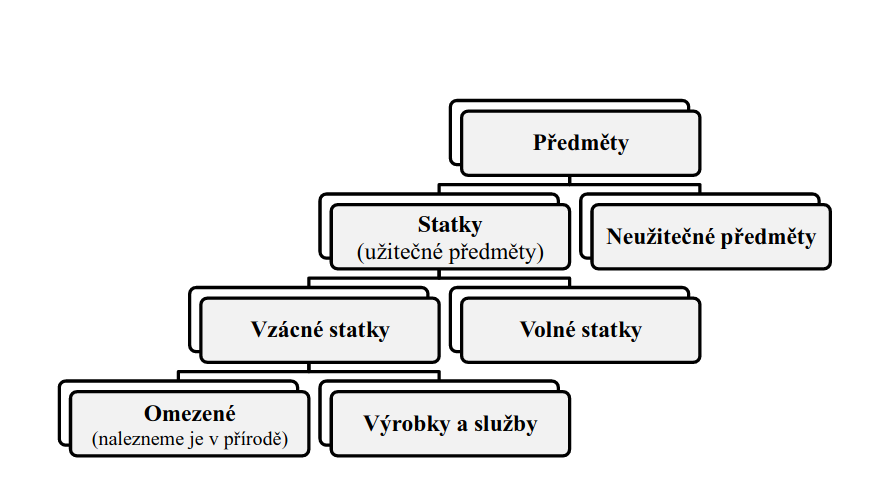
\includegraphics[width=16cm]{images/02_deleni.png}

\subsection{Výrobní faktory}
\begin{itemize}
    \item Práce (lidská činnost, přírodní zdroje -> užitečné statky, za to mzda)
    \item Půda (produkt přírody, není volný statek, i přírodní zdroje, např. nerosty)
    \item Kapitál (výsledek předchozí činnosti, hmotný nebo nehmotný, výsledkem jeho užití je zisk nebo úrok)
    \item Výrobní faktory jsou ve vlastnictví domácností a ty je pronajímají firmám za důchod. Za ten pak
    nakupují od firem statky.
\end{itemize}

\subsection{Hranice produkčních možností}
\begin{itemize}
    \item Je to křivka znázorňující různé kombinace statků nebo služeb, které mohou být vyrobeny s fixním množstvím výrobních faktorů při jejich efektivním využití.
    \item body na křivce znázorňují efektivní kombinace, body pod ní neefektivní, body nad ní nedosažitelné
\end{itemize}
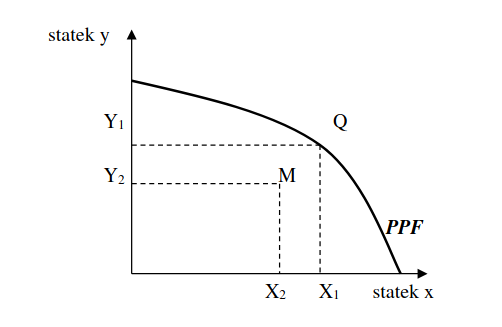
\includegraphics[width=16cm]{images/02_hranice_vyrobnich_moznosti.png}
\clearpage
\section{Vznik trhu. Definice trhu. Základní pravidla pro fungování tržní ekonomiky. Dělení trhů.}

\subsection{Vznik trhu}
\begin{itemize}
    \item Kvůli dělbě práce, díky němu je větší efektivita
    \item Předcházel mu barter (směna výrobků)
\end{itemize}

\subsection{Definice trhu}
\begin{itemize}
    \item Uspořádání, při kterém na sebe vzájemně působí prodávající a kupující, což vede ke stanovení cen 
    a~množství výrobků (či služeb)
    \item oblast ekonomiky, ve které dochází k směně činností mezi jednotlivými ekonomickými subjekty
    prostřednictvím směny zboží
\end{itemize}

\subsection{Základní pravidla pro fungování tržní ekonomiky}
\begin{itemize}
    \item dodržování smluv
    \item ochrana soukromého vlastnictví
    \item volný vstup na trhy
\end{itemize}

\subsection{Dělení trhů}
\begin{itemize}
    \item Podle územního hlediska:
    \begin{itemize}
        \item místní
        \item národní
        \item světový
    \end{itemize}
    \item podle počtu zboží, které na trhu sledujeme:
    \begin{itemize}
        \item dílčí (kupuje a prodává se na něm jediný druh zboží)
        \item agregátní
    \end{itemize}
    \item podle předmětu koupě a prodeje:
    \begin{itemize}
        \item trh výrobních faktorů (práce, půda, kapitál)
        \item trh peněz
        \item trh produktů (statků), pčítají se i služby
    \end{itemize}
\end{itemize}
\clearpage
\section{Ekonomický koloběh a funkce trhů. Úloha ceny v tržní ekonomice.}

\subsection{Ekonomický koloběh}
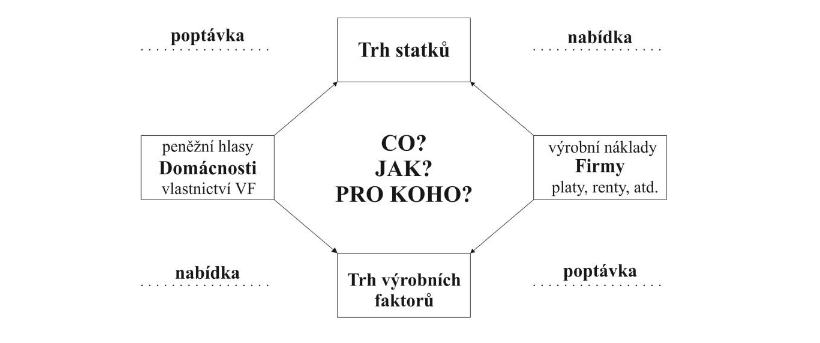
\includegraphics[width=16cm]{images/kolobeh.png}

\subsection{Funkce trhů}
\begin{itemize}
    \item Hledání odpovědí na otázky:
    \begin{itemize}
        \item \textbf{Co} vyrábět, rozhodováno peněžními hlasy (co se bude dobře prodávat)
        \item \textbf{Jak} vyrábět, soutěž mezi výrobci rozhoduje o nejlepším postupu
        \item \textbf{Pro koho} vyrábět, jak bude produkt rozdělen mezi jednotlivce nebo skupiny lidí
    \end{itemize}
    \item Dokáže na to odpovědět dokonale konkurenční trh, což je jen model
\end{itemize}

\subsection{Úloha ceny v tržní ekonomice}
\begin{itemize}
    \item Informační funkce - když se stane výrobní zdroj vzácnější, zvýší se cena
    \item Motivační funkce - Snaha ušetřit, spotřeba méně vzácných výrobků
    \item Alokační funkce - cenové informace -> přemístění výrobních zdrojů
\end{itemize}
\clearpage
\section{Kardinalistické pojetí chování spotřebitele (princip, definice mezního a celkového
užitku, rovnováha spotřebitele při spotřebě jednoho statku, přebytek spotřebitele,
rovnováha spotřebitele při spotřebě dvou a více statků) a odvození individuální
poptávky.}

\subsection{Princip}
\begin{itemize}
    \item Spotřebitel dokáže vyjádřit užitek v peněžních jednotkách
    \item Nakupuje, dokud se mezní užitek nerovná ceně statku
\end{itemize}

\subsection{Mezní užitek}
Přírůstek užitku s každou další pořízenou jednotkou statku, klesá s množstvím pořízených statků.

\subsection{Celkový užitek}
Součet všech mezních užitků, užitek ze všech pořízených statků. S každou další jednotkou roste,
ale \textit{rychlost přírůstku} se snižuje s každou další jednotkou (konkávní funkce).

\subsection{Rovnováha spotřebitele při spotřebě jednoho statku}
Nastává, pokud se tržní cena statku rovná meznímu užitku z nákupu tohoto statku.

\subsection{přebytek spotřebitele}
Jedná se o rozdíl celkové ceny, kterou byl zákazník ochotný zaplatit a ceny, za které byly opravdu statky nakoupeny. \\

\includegraphics[width=16cm]{images/05_prebytek_spotrebitele.png}

\subsection{Rovnováha spotřebitele při spotřebě dvou a více statků}
Musí platit, že poměr mezních užitků a cen jednotlivých statků je stejný pro všechny statky. \\
$\frac{MU_1}{P_1}=\frac{MU_2}{P_2}=\dots=\frac{MU_n}{P_n}$

\subsection{Odvození individuální poptávky}
V tomto pojetí je chápána jednoduše jako funkce mezního užitku (klesající), jen nemůže jít do záporných hodnot. (Končí mezním užitkem rovným nule.)

\clearpage
\section{Ordinalistické pojetí chování spotřebitele (princip, definice indiferenčního bodu,
indiferenční křivky a indiferenční mapy, definice a vztah pro mezní míra substituce ve
spotřebě, definice a rovnice linie rozpočtu, definice a vztah pro mezní míra substituce
ve směně, rovnováha spotřebitele, definice a vztah pro mezní míra substituce) a
odvození individuální poptávky.}
\clearpage
\section{Odvození tržní křivky poptávky, faktory ovlivňující poptávku, elasticita poptávky
(cenová, důchodová, křížová).}

\subsection{Odvození tržní křivky poptávky}
\begin{itemize}
    \item Platí, že celkové množství poptávaného statku je součet individuálních poptávaných množství, $Q=q_1+q_2+\dots +q_n$
    \item Postup:
    \begin{enumerate}
        \item Převést jednotlivé poptávky ze tvaru $p=-a\cdot q+b$ na tvar $q=\frac{-p+b}{a}$
        \item Sečíst jednotlivé poptávané množství, $Q=\frac{-p+b_1}{a_1}+\frac{-p+b_2}{a_2}+\dots+\frac{-p+b_n}{a_n}$
        \item Převést na tvar $D: P=-c\cdot Q+d$
    \end{enumerate}
\end{itemize}
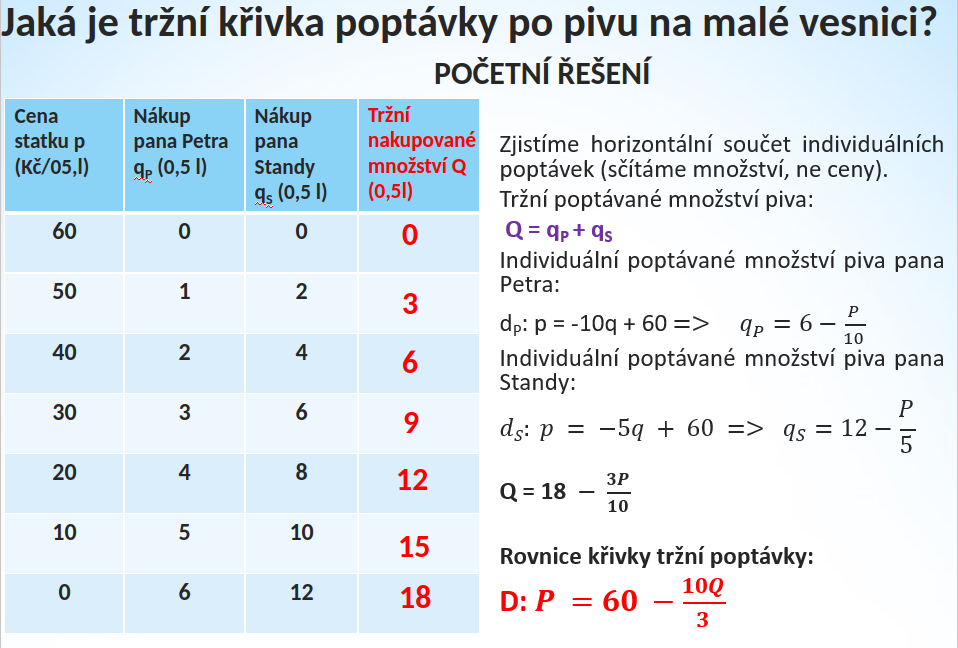
\includegraphics[width=16cm]{images/07_odvozeni_poptavky.png}

\subsection{Faktory ovlivňující poptávku}
\begin{itemize}
    \item Cenové faktory - posun po poptákové křivce
    \begin{itemize}
        \item Změna ceny statku
    \end{itemize}
    \item Necenové faktory - posun poptávkové křivky
    \begin{itemize}
        \item Změna důchodu spotřebitelů
        \item Změna ceny komplementů/substitutů
        \item Móda
        \item Očekávaná změna ceny zboží
    \end{itemize}
\end{itemize}

\subsection{Cenová elasticita poptávky}
\begin{itemize}
    \item $E_{PD}=\frac{\%\Delta Q}{\%\Delta P}$, kde $Q$ je množství a $P$ je cena
    \item Závislost mezi změnou množství a změnou ceny
    \item typy:
    \begin{enumerate}
        \item Dokonale elastická poptávka, $E_{PD}\rightarrow \infty$, poptávané množství nezávislé na ceně
        \item Elastická poptávka, $E_{PD}>1$, jednoprocentní změna ceny vyvolá větší než procentuálně jednotkovou změnu objemu poptávaného zboží (např. pokles ceny statku je doprovázen takovým zvýšením realizovaných prodejů, že se celkové tržby zvýší.
        \item Jednotkově elastická poptávka, $E_{PD}=1$ 
        \item Neelastická poptávka, $E_{PD} < 1$
        \item Dokonale neelastická poptávka, $E_{PD}=0$, poptávané množství se nemění.
    \end{enumerate}
\end{itemize}

\subsection{Důchodová elasticita poptávky}
\begin{itemize}
    \item $E_{ID}=\frac{\% \Delta Q}{\% \Delta I}$, kde $Q$ je množství a $I$ je výše důchodu
    \item citlivost reakce spotřebitele v nakupovaném množství statku na změnu důchodu
    \item typy:
    \begin{enumerate}
        \item Normální statek, $E_{ID}>0$
        \item Luxusní statek, $E_{ID}>1$, spotřeba roste rychleji než důchod
        \item Nezbytný normální statek, $0<E_{ID}<1$, spotřeba roste pomaleji než důchod, ale roste
        \item Podřadný statek, $E_{ID}<0$, spotřeba klesá se zvýšením důchodu
    \end{enumerate}
\end{itemize}

\subsection{Křížová elasticita}
\begin{itemize}
    \item $E_{CD}=\frac{\% \Delta Q_1}{\% \Delta P_2}$, kde $Q_1$ je množství jednoho statku a $P_2$ je cena druhého
    \item Závislost mezi změnou ceny jednoho statku a změnou poptávaného množství druhého
    \item typy:
    \begin{enumerate}
        \item Substituty, $E_{CD}>0$, cena jednoho se zvýší, koupíme radši jiný, zástupný statek
        \item Komplementy, $E_{CD}<0$, cena jednoho se zvýší, tak nechceme kupovat ani druhý,
        který se používá s prvním (např. zdrahne elektronika, bude se prodávat méně beden na PC)
    \end{enumerate}
\end{itemize}

\clearpage
\section{Chování výrobce – účetní a ekonomické pojetí nákladů, výnosů a zisku (explicitní
náklady, implicitní náklady, účetní zisk, ekonomický zisk, normální zisk), členění
nákladů v závislosti na velikosti objemu produkce (celkové náklad, fixní náklady,
variabilní náklady, mezní náklady, průměrné náklady, průměrné fixní náklady,
průměrné variabilní náklad) a příjmů (celkový příjem, průměrný příjem, mezní příjem).}
\clearpage
\section{Chování výrobce – krátkodobá rovnováha firmy, dlouhodobá rovnováhy firmy, bod
zvratu, bod zastavení činnosti firmy, odvození individuální nabídky.}

\subsection{Krátkodobá rovnováha firmy}
\begin{itemize}
    \item \textbf{Rovnováha} - stav, kdy aktéři, tvořící trh, nemají žádné důvody měnit
    své ekonomické chování. U firmy nastane při maximálním zisku.
    \item Platí $MC=MR$, graf na konci kapitoly
\end{itemize}

\subsection{Dlouhodobá rovnováha firmy}
\begin{itemize}
    \item na trzích se prosazuje tendence k nulovému ekonomickému zisku, $P=MR=MC=AR=AC$, cena se ustálí na bodu
    zvratu, v $P=AC_{min}$
    \item Kladný ekonomický zisk firem je přechodnou situací.
    
    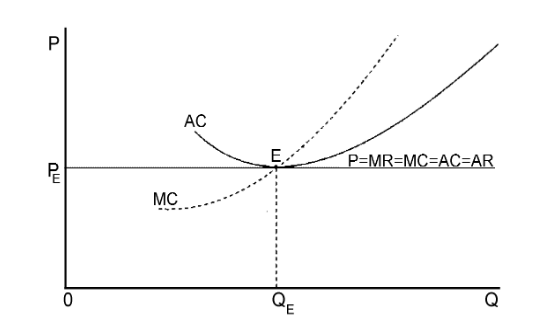
\includegraphics[width=15.5cm]{images/9_dlouhodoba.png}
\end{itemize}

\subsection{Bod zvratu}
\begin{itemize}
    \item Break Even Point
    \item množství produkce, od kterého začíná firma vytvářet zisk
    \item vyrovnání nákladů s příjmy
\end{itemize}

\subsection{Bod zastavení činnosti}
\begin{itemize}
    \item objem produkce, při kterém příjem nepokrývá ani variabilní náklady
    \item Je ekonomičtější nevyrábět vůbec, protože bude docházet k menším ztrátám 
    (ty budou rovné fixním nákladům)
\end{itemize}

\subsection{Odvození individuální nabídky}
Křivka individuální nabídky kopíruje část křivky mezních nákladů nad průsečíkem 
s~průměrnými variabilními náklady.

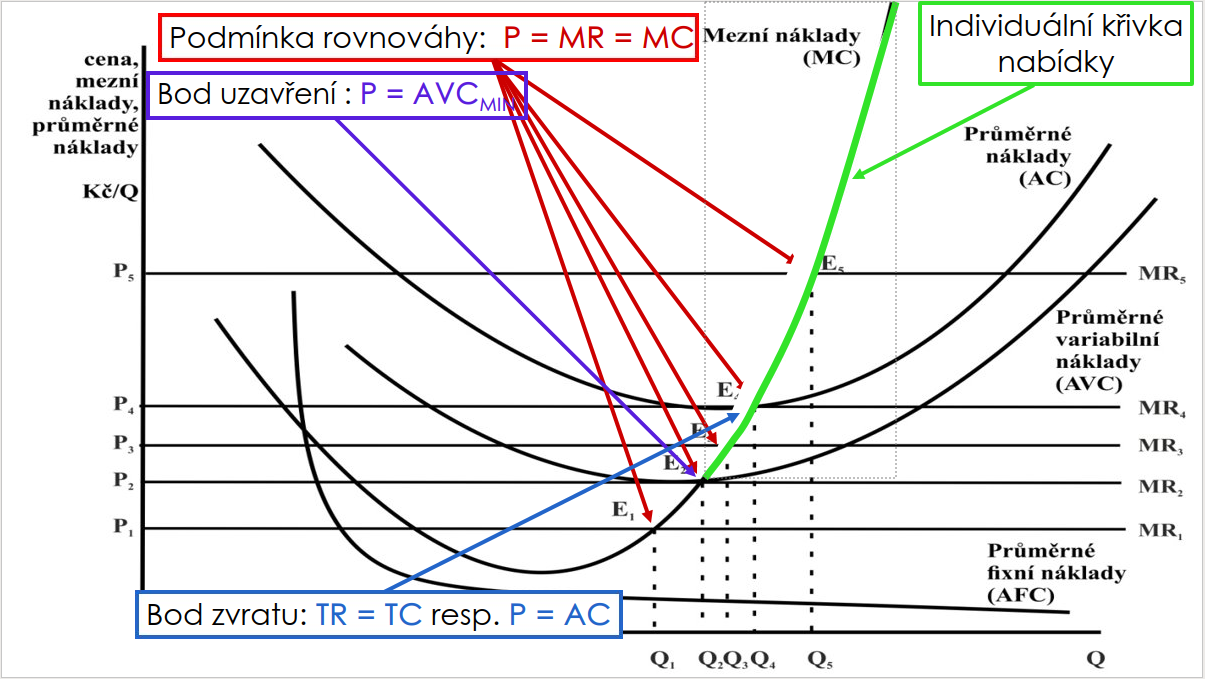
\includegraphics[width=16cm]{images/09_indiv_nabidka.png}
\clearpage
\section{Odvození tržní křivky nabídky. Faktory ovlivňující nabídku. Cenová elasticita nabídky.}

\subsection{Odvození}
\begin{itemize}
    \item Postup stejný jako u tržní poptávky, vycházíme z toho, že celkové nabízené množství je 
    součtem individuálních nabízených množství jednotlivých prodejců. $Q=q_1+q_2+\dots +q_n$
    \item Převedeme z tvaru $p=a\cdot q+b$ na $q=\frac{p-b}{a}$
    \item Sečíst,  $Q=\frac{p-b_1}{a_1}+\frac{p-b_2}{a_2}+\dots +\frac{p-b_n}{a_n}$
    \item Převést na tvar $S:P=c\cdot Q + d$
    \item Nebo graficky, sčítáme jednotlivé množství
\end{itemize}
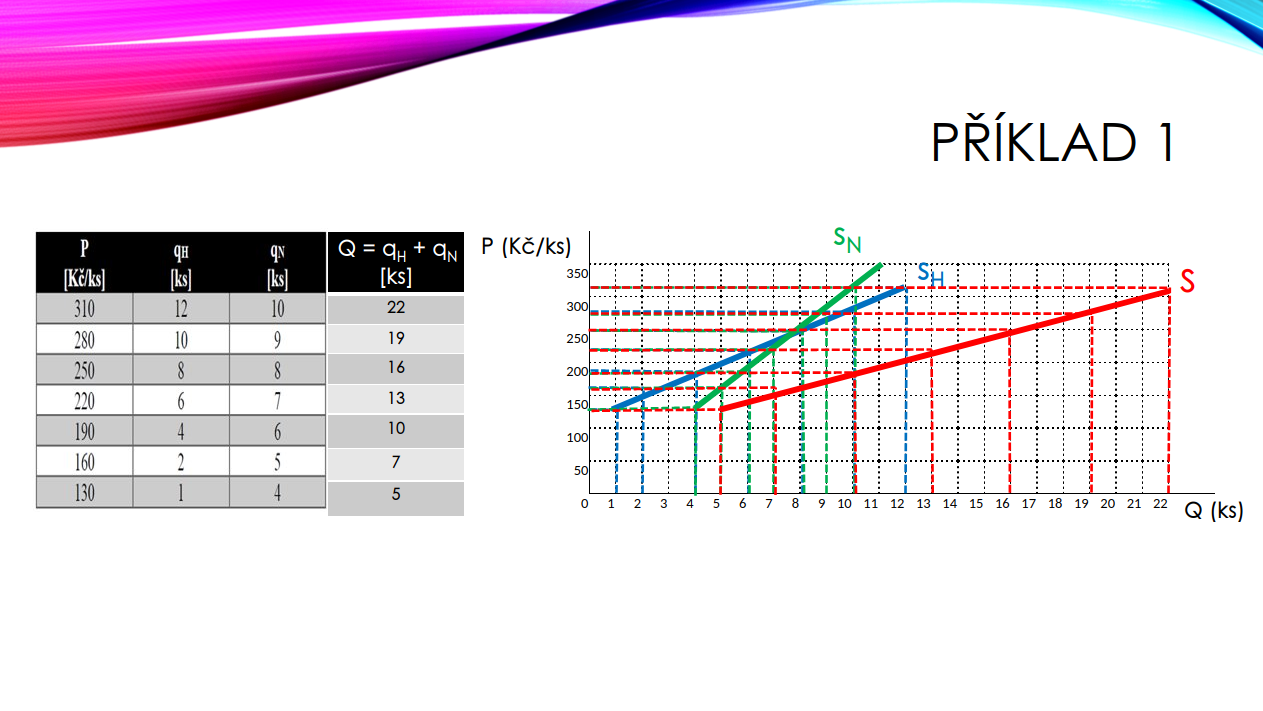
\includegraphics[width=16cm]{images/10_graficky.png}

\subsection{Faktory ovlivňující nabídku}
\begin{enumerate}
    \item Cenové faktory (posun po nabídkové křivce)
    \begin{itemize}
        \item Změna ceny
    \end{itemize}
    \item Necenové faktory (posun nabídkové křivky)
    \begin{itemize}
        \item Dokonalost technologií
        \item Očekávaná změna ceny
        \item Vstup nového prodejce na trh
        \item Změna ceny surovin
    \end{itemize}
\end{enumerate}

\subsection{Cenová elasticita}
\begin{itemize}
    \item $E_{PS}=\frac{\% \Delta Q_S}{\% \Delta P_S}$, kde $Q$ je množství a $P$ je cena
    \item Obdobně jako u poptávky
    \item $E_{PS}\rightarrow \infty$ - dokonale elastická nabídka, 
    \item $E_{PS}>1$ - elastická nabídka, při změně ceny obchodníci mění nabízený objem o větší část
    \item $E_{PS}<1$ - neelastická nabídka, obchodníci mění objem méně, než se mění cena
    \item $E_{PS}=0$ - dokonale neelastická nabídka
\end{itemize}
\clearpage
\section{Dokonalá konkurence (charakteristiky, tržní rovnováha a její efektivnost, přebytek
spotřebitele a přebytek výrobce, typy nerovnováhy).}

\subsection{Charakteristiky}
\begin{enumerate}
    \item \textbf{Velké množství prodávajících a nakupujících} (Velké množství nakupujících 
    umožňuje, aby firmy nebyly v područí jediného odběratele.)
    \item \textbf{Dokonalá informovanost kupujících} (splněno při burzách. V případě trhů 
    územně rozptýlených, jako jsou např. restaurační služby, hotely, cukrárny atp. nemívají
    kupující k dispozici všechny informace )
    \item \textbf{Homogenní produkt} (spotřebitel se rozhoduje o koupi výrobku výlučně podle
    ceny, nebere v úvahu jiná hlediska, např. kvalitu výrobku či pověst firmy. Tuto podmínku
    splňuje jen málo výrobků a služeb)
    \item \textbf{Volný vstup na trh} (a výstup z tohoto trhu) - spojeno s překážkami vstupu do odvětví.
    \begin{itemize}
        \item Žádné překážky vstupu (prodej textilu, webdesign, vedení účetnictví)
        \item Velké překážky vstupu (výroba elektřiny a její distribuce, či proniknutí
        na trh s operačními systémy pro PC) Typické překážky:
        \begin{itemize}
            \item vysoké fixní náklady
            \item kontrola zdrojů, nezbytných pro výrobu, jedinou firmou
            \item právní restrikce v podobě patentů, ochranných práv autorů
            \item udělení výsadního práva pro činnost firmy státem
        \end{itemize}
    \end{itemize}
    \item \textbf{Nulové náklady na změnu dodavatele} (pokud se rozhodne kupující změnit 
    dodavatele, tak jej tato změna nic nestojí žádné dodatečné náklady)
\end{enumerate}

\subsection{Tržní rovnováha}
Nastává, když se mezní užitek statku rovná mezním nákladům na jeho výrobu. 
Tržní rovnováha je pro ekonomickou realitu jev výjimečný.\\
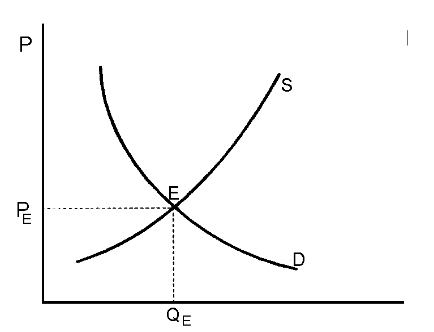
\includegraphics{images/11_trzni_rovnovaha.png}\\
\textbf{Efektivnost} spočívá v porovnání mezního užitku a mezních nákladů. Z toho vyplývá,
že společensky efektivní tržní produkcí je taková produkce statku, jejíž mezní užitek se rovná mezním
nákladům. Jinými slovy tržní rovnováha nastává v průsečíku křivky poptávky a křivky nabídky, neboť
tam se poptávané množství právě rovná nabízenému množství.

\subsection{Přebytek spotřebitele}
Je kumulativní rozdíl mezi částkou, kterou kupující byli ochotni zaplatit
za statek, a jeho skutečnou cenou na trhu.

\subsection{Přebytek výrobce}
Je rozdíl mezi celkovými příjmy firmy a součtem mezních nákladů.

\subsection{Typy nerovnováhy}
\begin{enumerate}
    \item \textbf{Tržní nedostatek} – poptávané množství převyšuje nabízené množství.
    Nedostatek vzniká, když je cena nižší než rovnovážná cena.
    \item \textbf{Tržní přebytek} – nabízené množství převyšuje poptávané množství. 
    Přebytek vzniká, když je cena vyšší než rovnovážná cena.
\end{enumerate}
\clearpage
\section{Nedokonalá konkurence (charakteristiky, rozdíly oproti dokonalé konkurenci, příčiny
vzniku.}

\subsection{Charakteristiky}
\begin{itemize}
    \item Nejsou splněné některé z podmínek dokonalé konkurence (velké množství 
    prodávajících a nakupujících, dokonalá informovanost kupujících, homogenní produkt,
    volný vstup na trh, nulové náklady na změnu dodavatele)
    \item Alespoň jeden prodávající (firma), který může ovlivnit tržní cenu
    \item Rozdílná ekonomická síla jednotlivých výrobců v důsledku koncentrace
    \item Méně efektivní než dokonalá konkurence, protože mezní náklady firem jsou menší 
    než mezní užitek jejich produkce
\end{itemize}

\subsection{Rozdíly oproti dokonalé konkurenci}
\begin{itemize}
    \item není v \uv{tvrdosti} konkurence, ale v cenové tvorbě
    \item Firmy na nedokonale konkurenčním trhu tvoří svou cenu, kdežto firmy na dokonale
    konkurenčním trhu cenu přijímají a ceně přizpůsobují nabízené množství.
    \item Individuální poptávková křivka klesá (a v případě monopolu je totožná s tržní 
    poptávkovou křivkou) a křivka mezních příjmů (MR) klesá rychleji než křivka poptávky.
    \item Na obou trzích, dokonalém i nedokonalém platí, že firmy maximalizují zisk při takové
    ceně, při které se mezní příjem rovná mezním nákladům (MR = MC).
\end{itemize}

\subsection{Příčiny vzniku}
\begin{enumerate}
    \item rozdílná ekonomická síla jednotlivých výrobců v důsledku koncentrace
    \item odlišné nákladové a poptávkové podmínky jednotlivých odvětví
    \item vysoké bariéry vstupu (např. vysoké fixní náklady)
    \item patentová práva
    \item cla
    \item vysoké dopravní náklady
\end{enumerate}
Patrně nejdůležitějším předpokladem vzniku nedokonale konkurenčního prostředí jsou odlišné
nákladové a poptávkové podmínky jednotlivých odvětví.
\clearpage
\section{Monopol (charakteristiky, typy monopolů, rovnováha monopolu, chování monopolu
oproti dokonalé konkurenci, efektivnost monopolu a cenová diskriminace, regulace
monopolu).}

\subsection{Charakteristiky}
Je to taková tržní situace, kdy na trh daného produktu dodává jediná firma. Tato
firma není vystavena konkurenci jiných firem, které by dodávaly stejný či podobný produkt.

\subsection{Typy monopolů}
\begin{enumerate}
    \item \textbf{Administrativní monopol} - Je-li vstup na trh vázán na povolení státu a dá-li stát 
    toto povolení pouze jediné firmě, získá tato firma administrativní monopol.
    \item \textbf{Přirozený monopol} - Přirozený monopol vzniká z důvodu přirozených bariér vstupu na trh.
    Tato situace nastává, když jsou dodávky zboží či služby vázány na určitou přenosovou síť. 
    stup na trh druhé firmě sice nikdo nezakazuje, ale brání jí v něm vysoké náklady, které by 
    musela vynaložit na vybudování vlastní přenosové soustavy, bez níž není možné zboží či služby dodávat.
\end{enumerate}

\subsection{Rovnováha monopolu}
Představuje takový objem produkce, při kterém firma maximalizuje zisk, přičemž musí být splněna
obecná podmínka MR = MC. Tento objem výroby je však menší než u dokonale konkurenční firmy 
za jinak stejných podmínek.

\subsection{Chování monopolu oproti dokonalé konkurenci}
Monopol nabízí menší množství a za vyšší cenu. Dosahuje ekonomického zisku, který nazýváme
monopolním ziskem. Platí-li spotřebitelé vyšší cenu, dochází k přerozdělování zisku na úkor 
spotřebitelů a ve prospěch monopolu. Monopol tedy vyvolává neefektivnost - poskytuje menší 
než optimální množství. Monopol tak způsobuje celospolečenské ztráty, tzv. společenské náklady monopolu.

\subsection{Efektivnost monopolu}
Efektivnost firem posoudíme, když porovnáme mezní náklady s mezním užitkem. Monopol
maximalizuje svůj zisk při takovém objemu výroby, při kterém se mezní příjem rovná
mezním nákladům (MR = MC). Objem výroby v odvětví s monopolem maximalizujícím zisk je tedy
nižší než objem výroby optimální pro společnost. Lze říci, že nedokonale konkurenční trhy jsou méně
efektivní než dokonale konkurenční trhy.\\
Skutečnost, že monopol disponuje určitou monopolní silou, mu umožňuje používat v cenové
strategii tzv. cenovou diskriminaci. Podstatou cenové diskriminace je stanovení rozdílných
cen stejných výrobků, aniž by k tomu vedly nákladové důvody (slevy pro studenty, děti, důchodce).

\subsection{Regulace monopolu}
\begin{enumerate}
    \item \textbf{Antitrustové zákonodárství} - omezují monopolizaci ekonomiky tím, že zakazují určité
    konkrétní chování firem (například jejich spojování, dohody o cenách apod.) - Úřad na
    ochranu hospodářské soutěže.
    \item \textbf{Ekonomická regulace} - pravidla nebo zákony, kterými stát ovlivňuje nebo
    kontroluje činnost firem. Ekonomická regulace se liší od cenové regulace tím, že neurčuje
    konkrétní ceny konkrétních výrobků, ale spíše stanoví pravidla pro cenovou tvorbu.
    \item \textbf{Daňová politika} - zvýšení daní sice snižuje zisky monopolů, ale neprojevuje se přímo
    ve velikosti vyráběného objemu produkce.
    \item \textbf{Převedení monopolu} do státního vlastnictví - je nástrojem, jehož použití ve větší míře než
    nástroje dosud zmíněné determinují širší okolnosti (politický systém, kultura, historie,
    tradice apod.).
    \item \textbf{Cenová regulace} - představují centralizované stanovení ceny konkrétních statků.
\end{enumerate}
\clearpage
\section{Oligopol (charakteristiky, typy oligopolů, rovnováha oligopolu s dominantní firmou)}
\clearpage
\section{Monopolistická konkurence (charakteristiky, krátkodobá rovnováha firmy,
dlouhodobá rovnováha firmy)}

\subsection{Charakteristiky monopolistické konkurence}
\begin{itemize}
    \item Mnoho firem
    \item Podobné, ale diferencované statky (např. mobilní telefony), jsou to vzájemné substituty
    \item Nízké bariéry vstupu do odvětví
    \item Žádná firma nemá dominantní postavení
\end{itemize}

\subsection{Krátkodobá rovnováha firmy}
\begin{itemize}
    \item Opět se vychází z $MR=MC$, z toho se zjistí objem a cena se dopočítá podle poptávkové křivky.
    \item $AR>AC$, monopolní zisk existuje
\end{itemize}
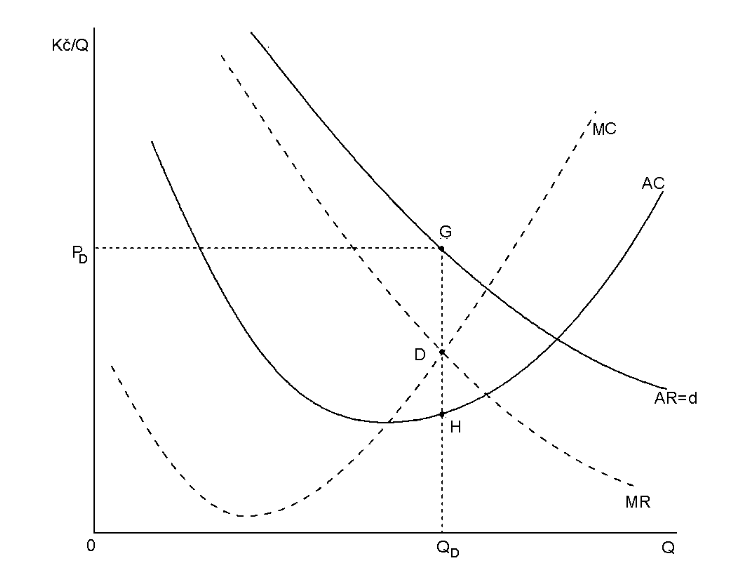
\includegraphics[width=16cm]{images/15_kratkodobe.png}

\subsection{Dlouhodobá rovnováha firmy}
\begin{itemize}
    \item Směřuje k nulovému monopolnímu zisku, protože vstupní náklady jsou nízké
    \item $AR\approx AC$
\end{itemize}
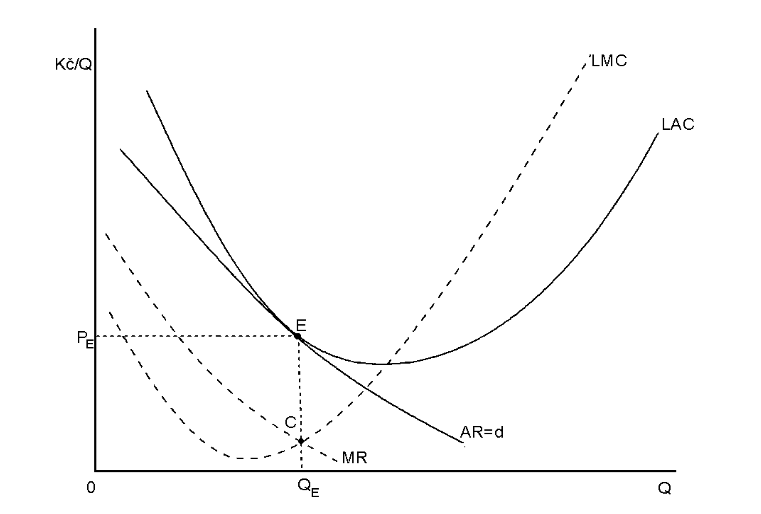
\includegraphics[width=16cm]{images/15_dlouhodobe.png}
\clearpage
\section{Trh výrobních faktorů (obecné a specifické výrobní faktory, produkční funkce a zákon
klesajících výnosů, poptávka a nabídka na trhu výrobních faktorů, rovnováha firmy na
trhu výrobních faktorů).}

\subsection{Obecné výrobní faktory}
\begin{itemize}
    \item Jsou to zdroje pro proces výroby.
    \item Základní skupiny:
    \begin{itemize}
        \item \textbf{práce} zahrnuje veškeré lidské zdroje, uplatnitelné ve výrobním procesu
        \item \textbf{půda} označuje v podstatě veškeré přírodní zdroje, ornou půdu, lesy, 
        zdroje nerostných surovin, moře, ovzduší apod.
        \item \textbf{kapitál} označuje výrobní faktory, které vznikají v průběhu výroby a jsou
        dále jako vstupy uplatňovány v další výrobě (suroviny, materiály, polotovary, energii, atd.)
    \end{itemize}
    \item Další obecné výrobní faktory:
    \begin{itemize}
        \item \textbf{technologie}
        \item \textbf{management}
    \end{itemize}
\end{itemize}

\subsection{Specifické výrobní faktory}
\begin{itemize}
    \item Je to konkrétní forma obecných výrobních faktorů.
    \item Např. konkrétní pozemky, kapitálové statky a pracovní profese, které jsou specializované 
    na výrobu konkrétních statků
\end{itemize}

\subsection{Produkční funkce}
\begin{itemize}
    \item Závislost produkce na množství výrobních faktorů
    \item Přírůstky produkce se nejdříve zvyšují a poté klesají.
    \item Klesá schopnost zvyšovat produkci, protože se projevuje nedostatek fixních faktorů.
    (To je \textbf{zákon klesajících výnosů})
    \item Např. produkční funkce na pile, kde je 5 strojů (fixní faktor) a variabilní počet dělníků:
\end{itemize}
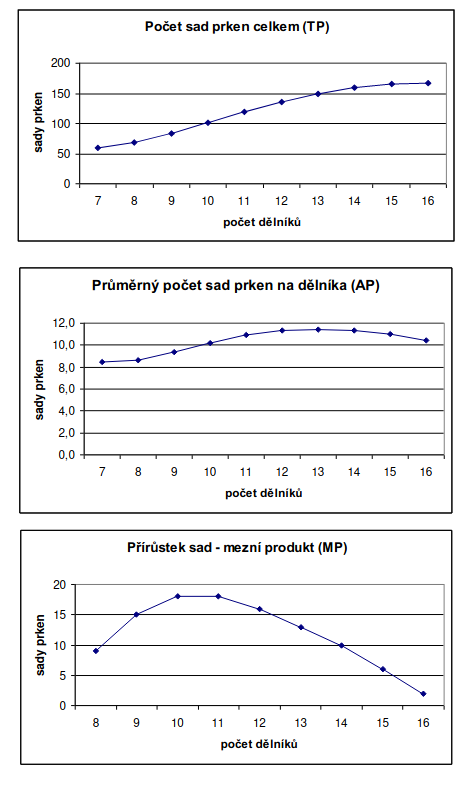
\includegraphics[]{images/16_prod_f.png}

\subsection{Poptávka na trhu výrobních faktorů}
\begin{itemize}
    \item Vůle maximalizovat zisk (největší výnosy a nejmenší náklady)
    \item Každá další jednotka výrobního faktoru:
    \begin{itemize}
        \item Mezní fyzický produkt (MP), dodatečný výstup zvýšením jednoho VF, při nezměnění ostatních
        \item Cena výrobku (P)
        \item Příjem z mezního produktu $MRP=MP\cdot P$
    \end{itemize}
\end{itemize}

\subsection{Nabídka na trhu výrobních faktorů}
\begin{itemize}
    \item Mezní náklady na výrobní faktor (MFC, Marginal Factor Costs), $MFC=\frac{\Delta TC}{\Delta VF}$,
    kde $\Delta TC$ je změna celkových nákladů a $\Delta VF$ je změna počtu výrobního faktoru
    \item Pokud panuje dokonalá konkurence, ceny výrobních faktorů udává trh a $MFC=P_F$, kde $P_F$ je
    cena za výrobní faktor
\end{itemize}

\subsection{Rovnováha firmy}
\begin{itemize}
    \item Rovnováha nastává, pokud platí $MRP=MFC$.
    \item Pokud $MRP>MFC$, firma najímá víc výrobního faktoru.
    \item Pokud $MRP<MFC$, firma snižuje nájem výrobního fkatoru.
\end{itemize}
\clearpage
\section{Trh práce (definice, nabídka práce, poptávka po práci, rovnováha na trhu práce,
nedokonalosti na trhu práce, nezaměstnanost).}

\subsection{Definice}
\begin{itemize}
    \item Rozhodování mezi volným časem a prací, určujeme si tím hodnotu volného času.
    \item Člověk nabízí svůj čas a za odměnu dostane mzdu. Ta je zároveň i důchodem.
\end{itemize}

\subsection{Nabídka práce}
\begin{itemize}
    \item Substituční efekt - při růstu mzdy chce člověk pracovat více
    \item Důchodový efekt - při růstu mzdy preferuje člověk svůj volný čas
    \item Projevují se oba, při různých výších mzdy, vzniká zpětně zakřivený průběh.
    \item Odvozena od poptávky po volném čase (kolik hodin člověk nechce jako volný čas, 
    tolik může pracovat).
\end{itemize}
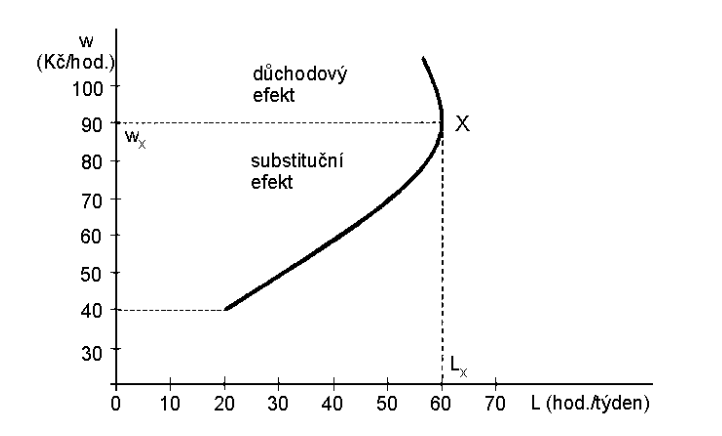
\includegraphics[width=16cm]{images/17_subs_duch_ef.png}

\subsection{Poptávka po práci}
\begin{itemize}
    \item Kolik práce firma najímá při různých cenách práce
    \item $MRP_L=MFC_L=w$, kde $MRP_L$ je příjem z mezního produktu práce, $MFC_L$ jsou
    mezní náklady na práci, $w$ je mzdová sazba 
\end{itemize}
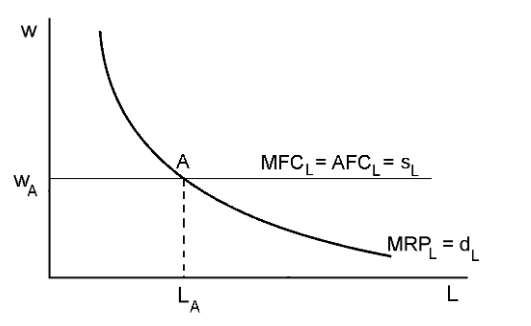
\includegraphics[width=16cm]{images/17_poptavka_po_praci.png}

\subsection{Rovnováha na trhu práce}
\begin{itemize}
    \item Průsečík poptávky a nabídky
    \item Mzdová sazba pod rovnovážným bodem vyvolá nedostatek pracovních sil (nezájem o práci).
    Jejich počet je dán úsečkou $CD$
    \item Nad bodem rovnováhy vzniká přebytek pracovních sil, nezaměstnanost, počet nezaměstnaných 
    je dán úsečkou $AB$.
\end{itemize}
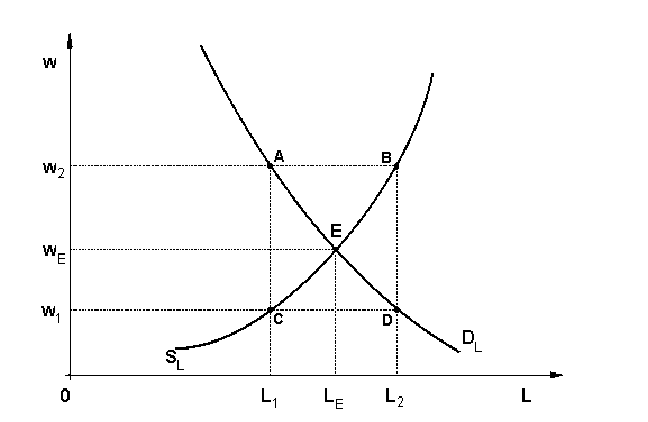
\includegraphics[width=16cm]{images/17_rovnovaha.png}

\subsection{Nedokonalosti na trhu práce}
\subsubsection{Na straně nabídky}
\begin{itemize}
    \item Strukturální různorodost - trhy nejsou konkurenční (lékaři a piloti se vzájemně nezastoupí)
    \item Diskrétnost nabídky - např. platové stupnice a omezení pracovní doby
    \item Mimoekonomické vlivy - aktivita odborů, regulační aktivita vlády
\end{itemize}
\subsubsection{Na straně poptávky}
\begin{itemize}
    \item Právní předpisy
    \item Kolektivní smlouvy
\end{itemize}

\subsection{Nezaměstnanost}
\begin{itemize}
    \item Kdo nemá práci a hledá ji
    \item Jak zjistit nezaměstnanost:
    \begin{enumerate}
        \item Registrovaná nezaměstnanost - nahlásí se na úřad práce,\\
        $$ Nezaměstnanost= \frac{Nezaměstnaní}{Všichni} \cdot 100 \% $$
        \item Pomocí výběrového šetření pracovních sil, nezaměstnaní podle ní jsou osoby starší 15 let, které nebyly zaměstnané, hledaly aktivně práci různými způsoby a byly připraveny k nástupu do práce nejpozději do 14 dnů.
    \end{enumerate}
    \item Metody se liší, protože ne každý registrovaný nezaměstnaný nepracuje (práce \uv{na černo}) 
\end{itemize}
\clearpage
\section{Trh kapitálu (definice, poptávka na trhu kapitálu, nabídka na trhu kapitálu, krátkodobá
rovnováha na trhu, dlouhodobá rovnováha na trhu, úroková míra).}
\clearpage
\section{Trh půdy (definice, poptávka na trhu půdy, nabídka na trhu půdy, rovnováha na trhu,
pozemková renta).}

\subsection{Definice}
\begin{itemize}
    \item Půda je konečný faktor
    \item Půda není homogenní (kvalita a poloha se různí)
    \item \textbf{Pozemková renta} je důchod plynoucí z vlastnictví půdy v průběhu jejího využívání.
    \item Kvalita a poloha mohou vytvořit přírodní monopol (prodává se dráž než by odpovídalo nákladům).
\end{itemize}

\subsection{Poptávka na trhu půdy}
\begin{itemize}
    \item Jako u ostatních výrobních faktorů je to klesající křivka. Za malou rentu poptáváme hodně půdy,
    za vysokou rentu málo.
\end{itemize}

\subsubsection{Nabídka na trhu půdy}
\begin{itemize}
    \item Nabízený objem je konstantní.
\end{itemize}

\subsection{Rovnováha na trhu půdy}
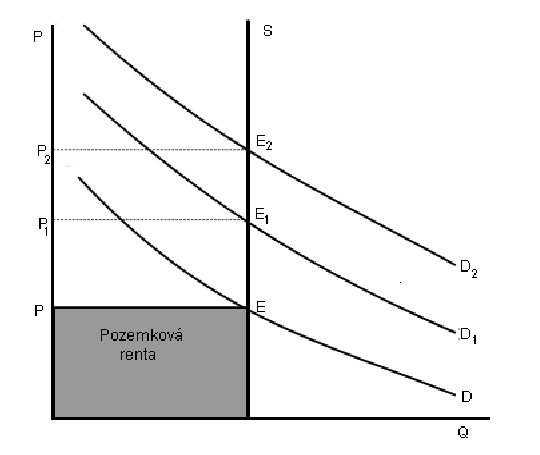
\includegraphics[]{images/19_rovnovaha.png}

\subsection{Pozemková renta}
\begin{itemize}
    \item Důchod plynoucí z vlastnictví půdy v průběhu jejího využívání
    \item Je to výnos z výrobního faktoru.
\end{itemize}
\clearpage
\section{Mikroekonomická politika státu a vládní selhání.}
\begin{itemize}
    \item Vliv státu na ekonomiku
    \item Nástroje hospodářské politiky:
    \begin{itemize}
        \item clo
        \item daně
        \item kvóty
        \item cenové regulace
        \item státní vlastnictví
        \item státní regulace (v sektoru veřejně prospěšných služeb, v dopravě, na finančních trzích,
        v zahraničním obchodu)
        \item antimonopolní politika (zakazuje určité druhy konkurenčního chování)
    \end{itemize}
    \item Řeší problémy jako inflace, nezaměstnanost
    \item \textbf{Podněty, které vedou orgány k zásahu:}
    \begin{itemize}
        \item neefektivní alokace výrobních faktorů a finální produkce
        \item přerozdělování příjmů
        \item konflikt mezi efektivitou a hodnotovým systémem společnosti
    \end{itemize}
\end{itemize}

\subsection{Neefektivní alokace výrobních faktorů a finální produkce}
\begin{itemize}
    \item Stát chce napomoct k efektivnější alokaci výrobních faktorů a finální produkce.
    \item Různé příčiny (nedokonalá konkurence, externality, nedokonalá informovanost)
    \item Mikroekonomický efekt - protimonopolní regulace
    \item Makroekonomický efekt - státní strukturální politika
\end{itemize}

\subsection{Přerozdělování příjmů}
\begin{itemize}
    \item Pokud stát nevnímá rozdělení příjmů trhem jako sociálně přijatelné
    \item Mikroekonomický efekt - vliv na dílčí trhy
    \item Makroekonomický efekt - vzájemné postavení ekonomických sektorů
\end{itemize}

\subsection{Konflikt mezi efektivitou a hodnotovým systémem společnosti}
\begin{itemize}
    \item Efektivní alokace může být v konfliktu s ostatními cíli společnosti
    \item Ochrana hodnotového  systému společnosti
    \item Např. prohibice
\end{itemize}

\subsection{Vládní selhání}
\begin{itemize}
    \item Činnost vlády negativně ovlivní rozdělení důchodů a nezlepší efektivnost
    \item Oblasti tržního selhání:
    \begin{itemize}
        \item čas (časové zpoždění)
        \item sledování vlastních zájmů
        \item vztah politiků k ekonomické teorii
        \item nevyužití politického kapitálu
    \end{itemize}
    \item Vláda chce maximalizovat zisk hlasů, ne ekonomickou prosperitu státu
\end{itemize}
\clearpage
\section{Zásahy státu do cen (spotřební daň, cenový strop, subvence k ceně).}
\clearpage
\section{Externality (definice, kladné externality, záporné externality, řešení externalit).}
\clearpage
\section{Veřejné statky (definice, rozhodování o veřejných statcích, úhrada za veřejný statek).}

\end{document}
